\subsubsection{Les flipbooks}

\paragraph{}
	Le principe d’un flipbook, ou folioscope en français, est de créer une suite d’images successives d’une scène par rapport à une trajectoire. Il suffira ensuite de mettre toutes ces images dans l’ordre les unes derrière les autres, et de les faire défiler rapidement pour avoir l’impression d’un rendu en relief et en mouvement. C’est également le principe des fichiers d’extension .GIF, qui font défiler une liste d’images.

        \footnotetext{OpenGL perspective projection : \url{http://www.3dcpptutorials.sk/index.php?id=2}}
        
\paragraph{}
	La création d’un flipbook est possible en créant une animation à l’aide d’un logiciel de manipulation d’objets 3D et en ne capturant que certaines images, par exemple avec Blender. Ainsi l’impression de ces images successives permet de réaliser un flipbook (cf. figure \ref{fig:flipbook}). En combinant par exemple avec le logiciel Gimp (outil d’édition et de retouche d’image) l’animation peut être obtenue en GIF. 

\begin{figure}[h!]
		\centering
		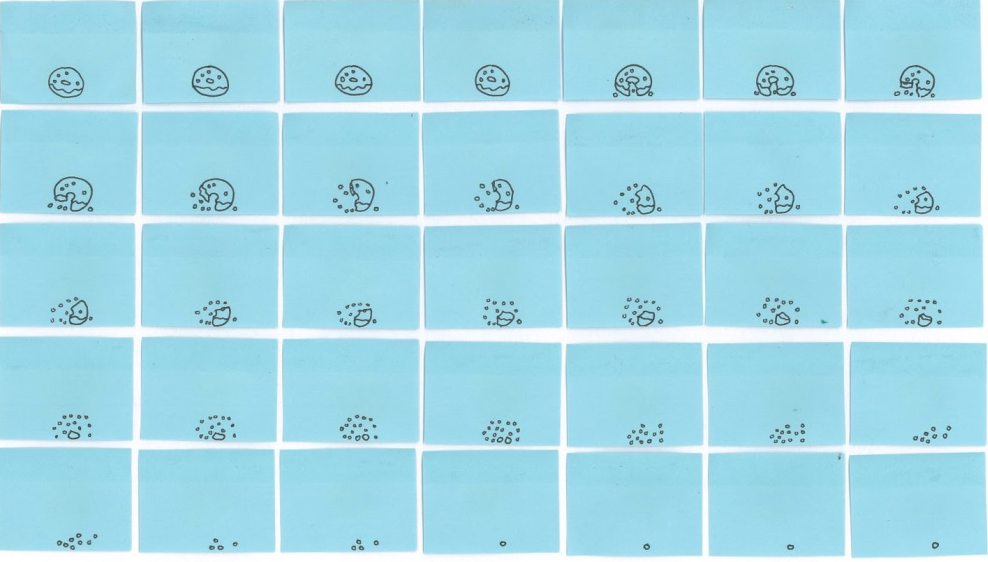
\includegraphics[scale=0.7]{flipbook.png}
		\caption{\label{fig:flipbook} Story-board d’un flipbook \protect \footnotemark }
\end{figure}
\footnotetext{\url{http://tracieliu.blogspot.fr/2010/08/flipbook-storyboard.html}}

\subsubsection{Les autostéréogrammes}	

\paragraph{}
	Un autostéréogramme est une image qui cache une visualisation en trois dimensions d’un objet. Cette image est construite de sorte qu'à chaque point de l'objet en trois dimensions soient associés deux points de l'image. L'utilisateur doit observer chaque point d'un couple de points avec un seul œil, ce qui donne l'illusion au cerveau d'observer deux images différentes avec les deux yeux et donc l'incite à traiter cette information comme l'observation d'un objet en trois dimensions, comme illustré par la figure \ref{fig:ppe_autostereogramme}.

\paragraph{}
	La visualisation en trois dimensions peut être difficile à obtenir, et demande une réelle gymnastique oculaire. Il faut pouvoir fixer le regard en avant ou en arrière de l’image, pour réussir à y voir l’objet caché. La plupart des autostéréogrammes sont observables en vision parallèle, c'est-à-dire qu'il faut faire le point au-delà de l'image pour pouvoir observer l'objet.

\begin{figure}[h]
  \centering
  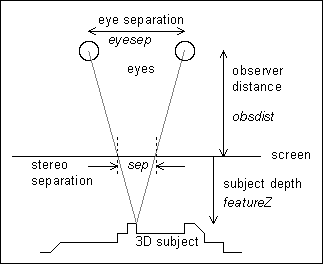
\includegraphics[scale=0.5]{./ppe_autostereogramme.png}
  \caption{Visualisation d’un autostéréogramme en vision parallèle \protect \footnotemark }
  \label{fig:ppe_autostereogramme}
\end{figure}

\footnotetext{\url{http://www.techmind.org/stereo/geometry.gif}}

\paragraph{}
	Pour générer un autostéréogramme, il faut utiliser une carte des profondeurs, ou carte de disparité, de l’objet à dissimuler. Cette carte s’obtient grâce à deux visions d’une même scène prises à deux endroits différents, et permet de mettre en avant les informations sur la profondeur de l’objet. Par exemple, la carte des profondeurs de la figure \ref{fig:carteProfondeur} a permis d’obtenir l’autostéréogramme de la figure \ref{fig:autostereogramme}.

\begin{figure}[h]
		\centering
		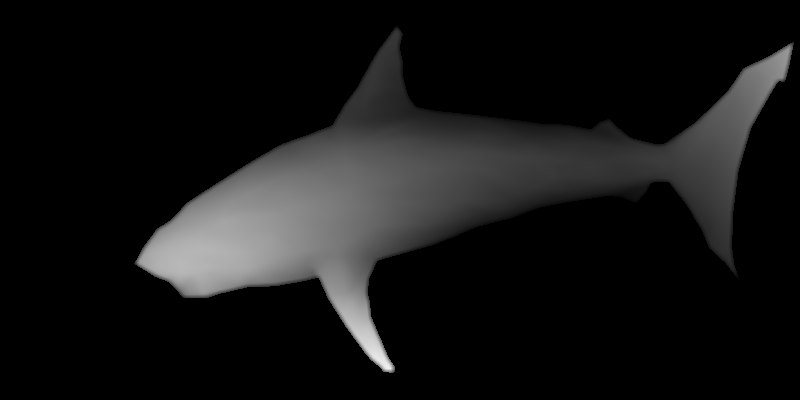
\includegraphics[scale=0.2]{carteProfondeur.png}
		\caption{\label{fig:carteProfondeur} Carte des profondeurs \protect \footnotemark }
\end{figure}
\footnotetext{\url{http://en.wikipedia.org/wiki/Autostereogram}}

\begin{figure}[h]
		\centering
		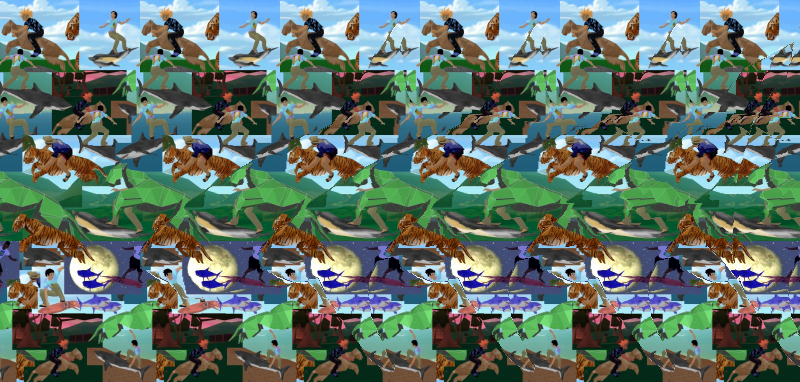
\includegraphics[scale=0.4]{autostereog.png}
		\caption{\label{fig:autostereogramme} Autostéréogramme obtenu \protect \footnotemark }
\end{figure}

\paragraph{}
Il existe des algorithmes de génération d’autostéréogrammes très simples , comme celui proposé par Gary Beene \cite{garybeene}. Cependant un algorithme aussi peu optimisé produit des autostéréogrammes défecteux, comportant par exemple des échos (répétition d'une partie de l'objet 3D) ou des artefacts (défaut de l'objet 3D observé).

\paragraph{}
Des algorithmes plus poussés ont été développés, comme celui présenté par Harold W. Thimbleby, Stuart Inglis et Ian H. Witten \cite{stereogram}, et celui proposé par W. A. Steer \cite{wasteer}, associés à une réalisation en C. Ils permettent la génération d’autostéréogrammes SIRDS (Single Image Random Dots Stereogram) à partir d’une image 2D. Ces articles présentent également des méthodes de correction de problèmes tels que l'écho ou la gestion des faces cachées (faces de l'objet tridimensionnel visibles par un seul œil). W. A. Steer propose de plus une méthode de génération d'autostéréogrammes utilisant un motif bitmap comme image de base plutôt qu'un nuage de points aléatoires, ce qui pallie à certaines limites des SIRDS comme le manque de détails et la grossièreté des surfaces courbes.
\footnotetext{\url{http://en.wikipedia.org/wiki/Autostereogram}}


\subsubsection{Les anaglyphes}

\paragraph{}
	Un anaglyphe est une image sur laquelle on superpose deux vues, si possible différentes, d’une scène. La meilleure distance entre ces deux visions est la même que celle entre les deux yeux, afin que le cerveau puisse recréer la même vision en trois dimensions que dans la réalité.
	
\paragraph{}
	Les anaglyphes les plus fréquents sont les anaglyphes dits rouge-cyan. Ils se nomment ainsi car ils sont constitués d’une image sur laquelle on passe un filtre magenta, et une autre avec un filtre cyan (cf. figure \ref{fig:anaglyph}). Pour pouvoir visualiser le relief sur une telle image, on utilise une paire de lunettes rouge-cyan, dont chaque verre est un filtre pour l’une des deux couleurs de l’image. Le plus souvent, le filtre magenta est placé sur l’œil gauche, le cyan sur l’œil droit. En regardant l’image, l’œil gauche ne verra alors que la composante cyan, et inversement pour l’œil droit. Les deux images ayant un léger décalage, le cerveau va percevoir l’image comme si elle était en trois dimensions. Les anaglyphes rouge-cyan sont principalement intéressants sur des images en noir et blanc. En effet, quand il s’agit d’images en couleur, celles-ci sont souvent détériorées par l’usage des filtres, car les couleurs possèdent généralement de plusieurs composantes. A l’inverse, quand l’image est en nuances de gris, l’image n’est pas modifiée, juste mise en relief. Plusieurs types d'algorithmes existent pour créer des anaglyphes depuis des paires d'images. Ils se différencient par la qualité de l'anaglyphe en sortie en diminuant le nombre d'artefacts \cite{steteroAnaglyph} ou en améliorant le rendu pour l'impression \cite{printAnaglyph} par exemple.

\begin{figure}[h]
		\centering
		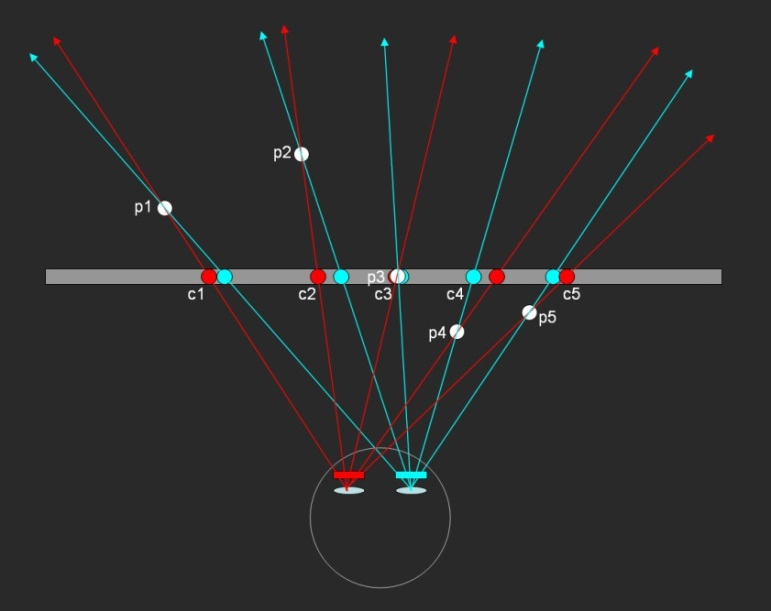
\includegraphics[scale=0.8]{anaglyph.png}
		\caption{\label{fig:anaglyph} Le décalage de la partie rouge et cyan permet à l’œil de percevoir l’image non plus dans un plan XY mais dans l’espace \protect \footnotemark }
\end{figure}
\footnotetext{\url{http://www.david-romeuf.fr/3D/Anaglyphes/TCAnaglypheLSDubois/TransformationCouleursPourAnaglyphe.html}}



[IMAGE D'UN ANAGLYPHE]	
	
